% EPL master thesis covers template
\documentclass{EPL-master-thesis-covers-EN}

% Please fill in the following boxes
% Title of the thesis
\title{Main title of the master thesis (possibly split on several lines)}

% Subtitle - remove this line if not applicable
\subtitle{Optional subtitle}

% Name of the student author(s)
\author{Michele \textsc{Cerra}}
%\secondauthor{Firstname \textsc{Lastname}}		% remove if not applicable
%\thirdauthor{Firstname \textsc{Lastname}}			% remove if not applicable

% Official title of the master degree (copy/paste from list below)
% Master [120] in Biomedical Engineering
% Master [120] in Chemical and Materials Engineering
% Master [120] in Civil Engineering
% Master [120] in Computer Science
% Master [120] in Computer Science and Engineering
% Master [120] in Cybersecurity
% Master [120] in Data Sciences Engineering
% Master [120] in Data Science: Information technology
% Master [120] in Electrical Engineering
% Master [120] in Electro-mechanical Engineering
% Master [120] in Mathematical Engineering
% Master [120] in Mechanical Engineering
% Master [120] in Physical Engineering
% Master [60] in Computer Science
% Specialised master in nanotechnologies
% Specialised master in nuclear engineering
\degreetitle{Master [120] in Computer Science and Engineering}

% Name of the supervisor(s)
\supervisor{Benoît \textsc{Macq}}
%\secondsupervisor{Firstname \textsc{Lastname}}		% remove if not applicable
%\thirdsupervisor{Firstname \textsc{Lastname}}		% remove if not applicable

% Name of the reader(s)
\readerone{Alexandre \textsc{Berger}}
%\readertwo{Firstname \textsc{Lastname}}			% remove if not applicable
%\readerthree{Firstname \textsc{Lastname}}			% remove if not applicable
%\readerfour{Firstname \textsc{Lastname}}			% remove if not applicable
%\readerfive{Firstname \textsc{Lastname}}			% remove if not applicable

% Academic year (update if necessary)
\years{2022--2023}

% Document
\begin{document}
  % Front cover page
  \maketitle

  \addcontentsline{toc}{chapter}{Abstract}
  \chapter*{Abstract}
  
  \addcontentsline{toc}{chapter}{Acknowledgments}
  \chapter*{Acknowledgments}

  \tableofcontents

  \addcontentsline{toc}{chapter}{Introduction}
  \chapter*{Introduction}
  %A biomarker for epileptogenesis is an objectively measurable characteristic of a biological process that reliably identifies the development, presence, severity, progression, or localization of an epileptogenic abnormality. An epileptogenic abnormality refers to the pathophysiological substrate(s) responsible for the initiation and/or maintenance

  \chapter{Theoretical background}
  \section{Magnetic Resonance Imaging}

\section{Diffusion-Weighted MRI}

\section{DW-MRI Microstructural Models}


  \chapter[Epilepsy]{Epilepsy disease}
  \section{Overview of Epilepsy}
Epilepsy is a disorder of the brain characterized by a lasting predisposition to generate spontaneous epileptic seizures, and has a numerous neurobiological, cognitive, and psychosocial consequences \cite{defEpilepsy}.
Epilepsy affects over 50 million people worldwide, making it one of the most common neurological diseases globally \cite{WHO}. Over 75\% of those with active epilepsy are untreated \cite{defeating_epilepsy}.

Epilepsy incidence is bimodally distributed with two peaks: the first in the pediatric population less than 5 years old, and the second in people over the age of 50 years. The incidence is higher in low-income countries than high-income countries, thanks a contribution of poor hygiene, poor basic sanitation and higher risk of infection \cite{THIJS2019689}.
Regardless the geographical location, the prevalence of active epilepsy is usually between 4 and 12 per 1000, with a risk factor that varies with age \cite{Fiest296}.

The risk of death for a person with epilepsy is increased compared with the risk for the general population. Mortality in epilepsy can be divided into direct (eg, status epilepticus, injuries, SUDEP \cite{Langan211}) or indirect (eg, suicide, drowning) disease-related death \cite{Devinsky779}. 

\noindent SUDEP (Sudden Unexpected Death in Epilepsy) is one of the causes of epilepsy-related death, it refers to a death in a patient with epilepsy that is not due to trauma, drowning, status epilepticus, or other known causes but for which there is often evidence of an associated seizure \cite{Nashef1997}. The exact cause of SUDEP is not well understood, but it is thought to be related to abnormalities in the electrical activity of the brain during seizures, which can affect the heart and breathing \cite{Devinsky2011}. SUDEP is most commonly seen in people with uncontrolled seizures, particularly those with generalized tonic-clonic seizures \cite{Devinsky2011}

Epilepsy rarely stands alone and the presence of comorbidities is the norm: more than 50\% of people with epilepsy have one or several additional medical problems \cite{THIJS2019689}. These comorbidities not only include include psychiatric conditions (e.g. depression, anxiety disorder, psychosis, autism spectrum disorder, dementia), but even somatic conditions (e.g. type 1 diabetes, arthritis, digestive tract ulcers) \cite{yuen2018epilepsy}.

  \subsection*{Definitions}
    \subsubsection*{Epilepsy}
    The given definition of Epilepsy is usually practically applied as having two unprovoked seizures occurring more than 24h apart. But the International League Against Epilepsy (ILAE) proposed that epilepsy be considered to be a disease of the brain by any of the following conditions: \cite{defEpilepsy}

    \begin{itemize}
      \item At least two unprovoked seizures occurring more than 24h apart;
      \item A single unprovoked seizure if recurrence risk is high (>60\% over the next 10 years);
      \item Diagnosis of an epilepsy syndrome.
    \end{itemize}
    \subsubsection*{Seizure}
    An epileptic seizure is the clinical manifestation of an abnormal, excessive, purposeless and synchronized electrical discharge in the neurons, that may leads to involuntary movement that may involve a part of the body (partial) or the entire body (generalized) \cite{WHO}. Another type of generalized seizure is the absence seizure which is accompanied by loss of consciousness with periods of blanking out or staring into space for a few seconds \cite{AbsenceS25:online}.

  \subsection*{Pathophysiology}
  A seizure can be conceptualized as occurring when there is a distortion of the normal balance between excitation and inhibition within a neural network \cite{pathophysiology}. 
  
  In focal epilepsies, focal functional disruption results in seizures beginning in a localized fashion in one hemisphere,
  commonly limbic or neocortical, which then spread by recruitment of other brain areas. The site of the focus and the speed and extent of spread determine the clinical manifestation of the seizure \cite{DUNCAN2006, classification}. For generalized epilepsies, epileptogenic networks are widely distributed, involving thalamocortical structures bilaterally \cite{classification}.

  The imbalance between excitation and inhibition resulting in epileptogenic networks is not necessarily only an increase of excitation or a loss of inhibition; an aberrant increase in inhibition can also be pro-epileptogenic in some circumstances, such as absence seizures \cite{pinault2005cellular} or limbic epilepsies in the immature brain. \cite{galanopoulou2008gabaa}

  \subsection*{Types of epilepsy}
  Classification is made at three levels: seizure type, epilepsy type, and epilepsy syndromes. \cite{classification}
    \subsubsection*{Seizure type}
    Seizures are first classified by onset as either focal, generalized or unknown as shown in Figure \ref{fig:Classification of epileptic seizures}.
    \begin{itemize}
      \item Focal Onset: Usually limited to a specific region of the brain, called the focus. Level of awareness subdivides focal seizure in those with retained awareness and impaired awareness. Retained awareness means that the person is aware of self and environment during the seizure, even if immobile. In addition, focal seizures are sub-grouped as those with motor and non-motor manifestation.
      \item Generalized Onset: Affects most or all of the brain. Typically congenital and occurs simultaneously in both hemispheres of the brain. They are almost always accompanied by impaired awareness. Generalized seizures are divided into motor and non-motor (absence) seizures.
      \item Unknown: It is the case in which the onset is missed or obscured. 
    \end{itemize}

    \begin{figure}[h]
      \centering
      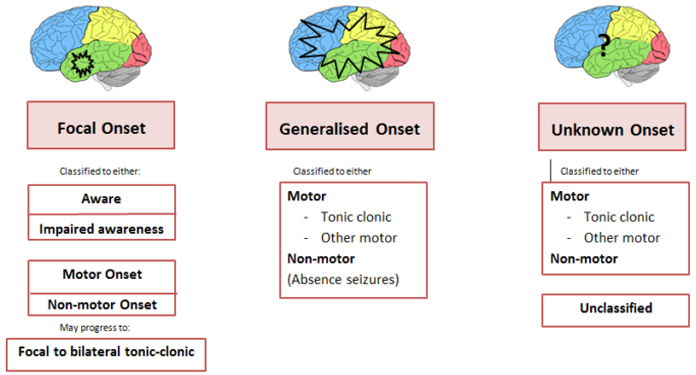
\includegraphics[width=0.8\textwidth]{images/seizureTypes.png}
      \caption{The International League Against Epilepsy.\cite{Scheffer2017}}
      \label{fig:Classification of epileptic seizures}
    \end{figure}
  
    % TODO [thesis Danthine2021]
    \subsubsection*{Epilepsy type}
    Epilepsies are divided into: focal, generalized, combined generalized and focal, and unknown as shown in Figure \ref{fig:Classification of epilepsies}. The category combined epilepsy is used for those presenting both seizure types.

    \begin{figure}[h]
      \centering
      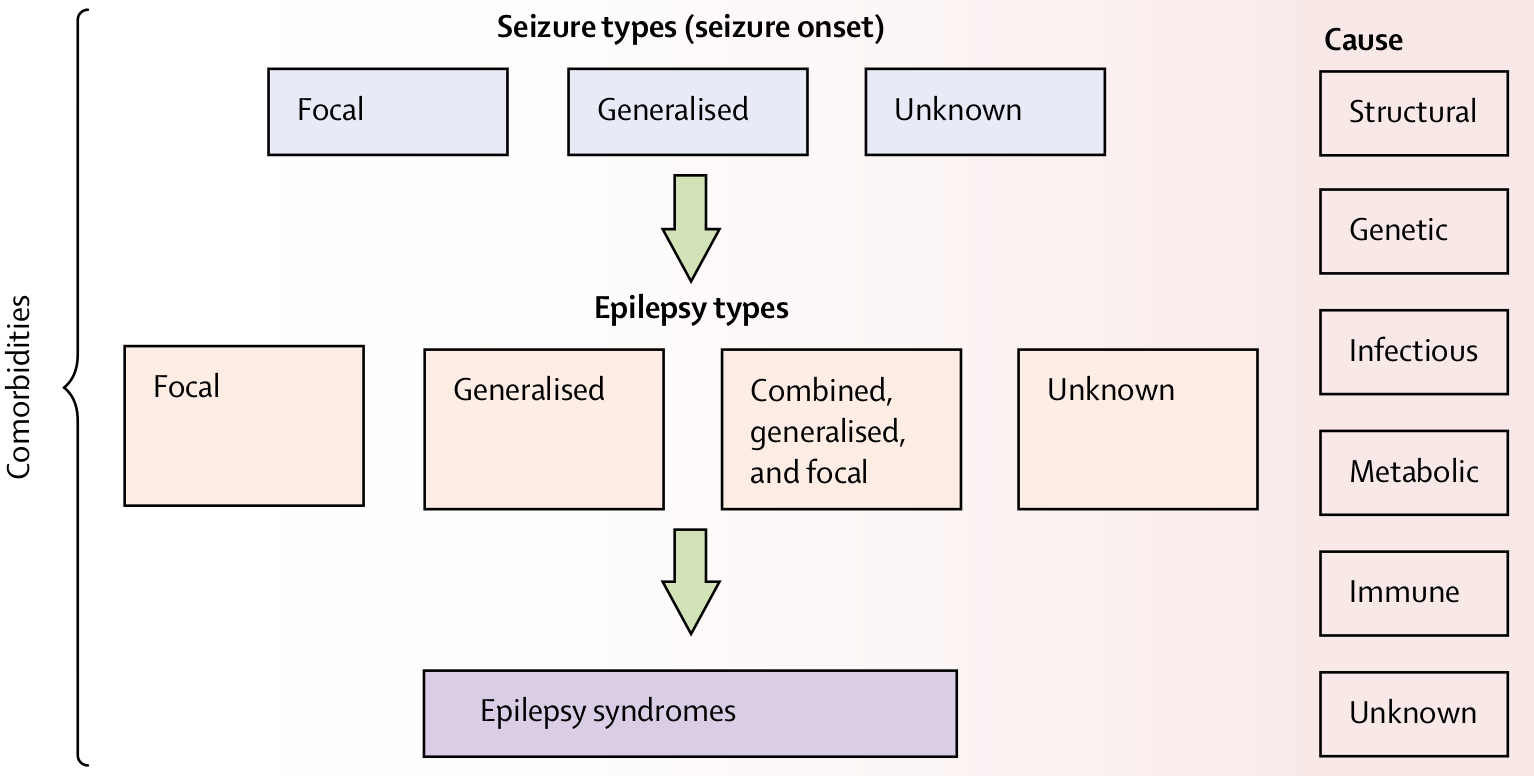
\includegraphics[width=0.8\textwidth]{images/epilepsyTypes.png}
      \caption{The International League Against Epilepsy.\cite{THIJS2019689, classification}}
      \label{fig:Classification of epilepsies}
    \end{figure}
  
  % TODO [thesis Danthine2021]
  \subsection*{Causes of epilepsy}
  Each possible type of the classification can have different causes as shown in \ref{fig:Classification of epilepsies} : structural, genetic, infectious, metabolic, immune and unknown. Established acquired causes include serious brain trauma, stroke, tumours, and brain problems resulting from a previous infection. \cite{THIJS2019689, classification}

  \subsection*{Treatments}
  For most of the people with epilepsy Antiepileptic Drug(AEDs) constitute the first line treatment. However, it has been reported that AEDs are effective in only 60-70\% of individuals, a percentage that is further reduced in low-income countries. \cite{DUNCAN2006}.

  Up to a third of all individuals with epilepsy are refractory to AEDs \cite{SpencerHuh2008}. Drug-resistant epilepsy is assumed after the "failure of adequate trials of two tolerated, appropriately chosen and used at correct dosage antiseizure drug schedules to achieve sustained seizure freedom" \cite{drug_resist}. In those cases alternative non-pharmacological treatments including surgery and neurostimulatory interventions should be considered.
  When surgery is not possible because of the presence of multifocal or generalized epilepsy or whenever the epileptogenic focus lies in eloquent cortex that cannot removed, neurostimulation techniques are palliative options \cite{Englot2013}.

  Three neurostimulation devices are approved by the Food and Drug Administration (FDA) for the treatment of drug resistant epilepsy \cite{wong2019comparison}.
  \begin{itemize}
    \item VNS is a device placed under the skin and sends intermittent signals to the vagus nerve. It is not a brain surgery and is approved for the treatment of epilepsy when surgery is not possible. \cite{Neuromod7:online}
    \item RNS is a device that can record seizure activity directly from the brain and delivers stimulation to stop seizures. RNS is implanted near the seizure focus on the skull. It delivers pulses only when detects abnormal activity in the seizure focus. \cite{Neuromod7:online}
    \item DBS sends signals to brain electrodes to stop signals that trigger a seizure. The connected DBS electrodes are typically placed inside the thalamus, and the electrical pulses are delivered constantly or not. \cite{Neuromod7:online}
  \end{itemize}

  \begin{figure}[h]
    \centering
    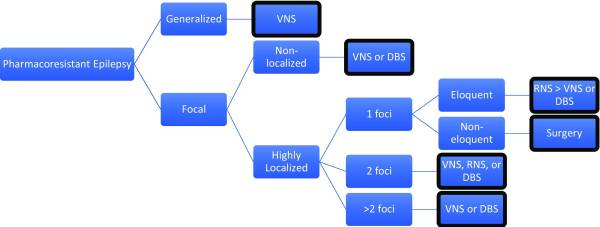
\includegraphics[width=0.8\textwidth]{images/WongMani2019.jpeg}
    \caption{The following shows a general algorithm for efficacious device selection based on mechanism of action and focality. Other considerations (side effects, device features, and patient preferences) also drive device selection but are not captured in this flowchart. \cite{wong2019comparison}}
    \label{fig:Decision algorithm}
  \end{figure}

\section{Vagus Nerve Stimulation}
Vagus Nerve Stimulation (VNS) showed positive effects in multiple other medical conditions, including essential tremors gastroparesis \cite{KRAHL2004135}, chronic tinnitus, stroke, post-traumatic stress disorder \cite{HAYS2013275}, chronic pain, Parkinson's disease, eating disorders, multiple sclerosis, migraine and Alzheimer's disease \cite{BRONCEL202037, BeekwilderBeems2010}.

VNS was implanted first time in four epilepsy patients by Penry and Dean in 1988 \cite{Penry1990}. After several large clinical studies, it was approved for seizures by the European Community in 1994 and FDA in 1997. Clinical trials demonstrate that 24 to 48 months after the implantation of the device, 60\% of patients were considered as responders and 8\% of implanted patients became seizure free \cite{Englot2016}. Responders to VNS will be defined as those who experience 50\% or greater reduction in seizure frequency after VNS \cite{IBRAHIM2017634}. Although VNS is used in clinical practice the exact mechanistic of its effect in modulating seizures remain poorly understood.

VNS consists of a device implanted in the upper left thoracic region with a helical electrode placed around the left cervical nerve, which delivers intermittent electrical impulses to activate the vagus nerve \ref{fig:Vagus Nerve Stimulation}.
Studies in the dog show that right-sided VNS results in a greater degree of bradycardia as compared to the left-sided VNS, because right vagus nerve innervates more densely in the heart \cite{ardell1986selective}. Because on those studies VNS is indicated for use only in stimulating the left vagus nerve.

Side effects of VNS are commonly limited to coughing and/or hoarseness of the voice. In a study, voice alternation was reported in 66\% of patients on high stimulation and in 30\% on low stimulation and cough was reported in 45\% of patients. \cite{ben2001vagus} To avoid cardiac side effects, a cuff electrode in most cases is implanted on the left vagal nerve.

\begin{figure}[h]
  \centering
  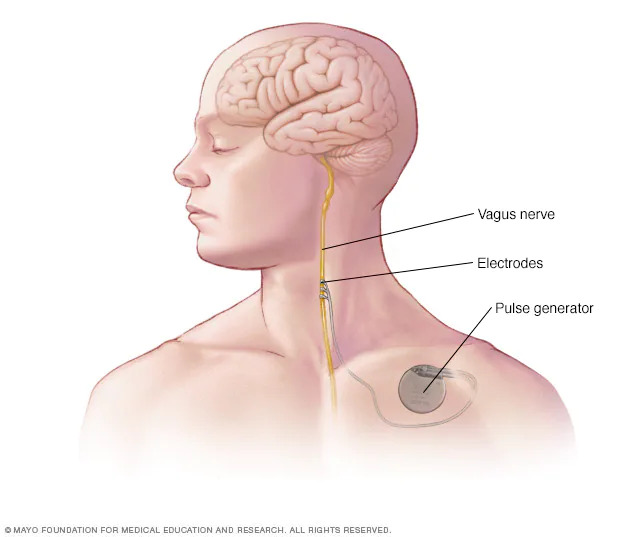
\includegraphics[width=0.7\textwidth]{images/vagus_nerve_stimulation.jpg}
  \caption{Components of the VNS system. \cite{MayoClinic}}
  \label{fig:Vagus Nerve Stimulation}
\end{figure}

  \subsection*{Vagus Nerve Anatomy and Connections}
  The vagal nerve (VN) is the longest cranial nerve and exerts a wide range of effects on the body. It comprises two nerves, the left and right vagus nerves and comprises both sensory and motor fibers.
  The vagal nerve is a mixed nerve made up of 75\% sensory(afferent) fibers responsible for the side effects observed (e.g. coughing, difficulties od swallowing, voice modification effects), and 25\% efferent fibers which mainly send feedback from heart, lungs, stomach and upper bowel.  \cite{BonazSinniger2017}.

  The majority of vagus nerve fibers are comprised of afferents and project to the nucleus tractus solitarius (NTS), which in turn sends fibers to other brainstem nuclei important in modulating the activity of subcortical and cortical circuitry, as shown in Figure \ref{fig:Vagus Afferent Network}. This vagus afferent network (VagAN) is
  thought to be the neural substrate of VNS efficacy \cite{HanchemWongIbrahim2018}. 
  The NTS receives direct inputs from the VN and projects to others brainstem nuclei: the locus coeruleus (LC), dorsal raphe nucleus (DRN), and parabranchial nucleus (PBN) \cite{RICARDO19781}. The functional importance of NTS connectivity in modulating seizure activity is further borne out by findings in rats that increased inhibitory gamma-aminobutyric acid (GABA) signaling or decreased excitatory glutamate signaling within the NST, reduces the susceptibility to chemically induced limbic motor seizures \cite{GABA}.

  \begin{figure}[h]
    \begin{minipage}[c]{0.5\textwidth}
      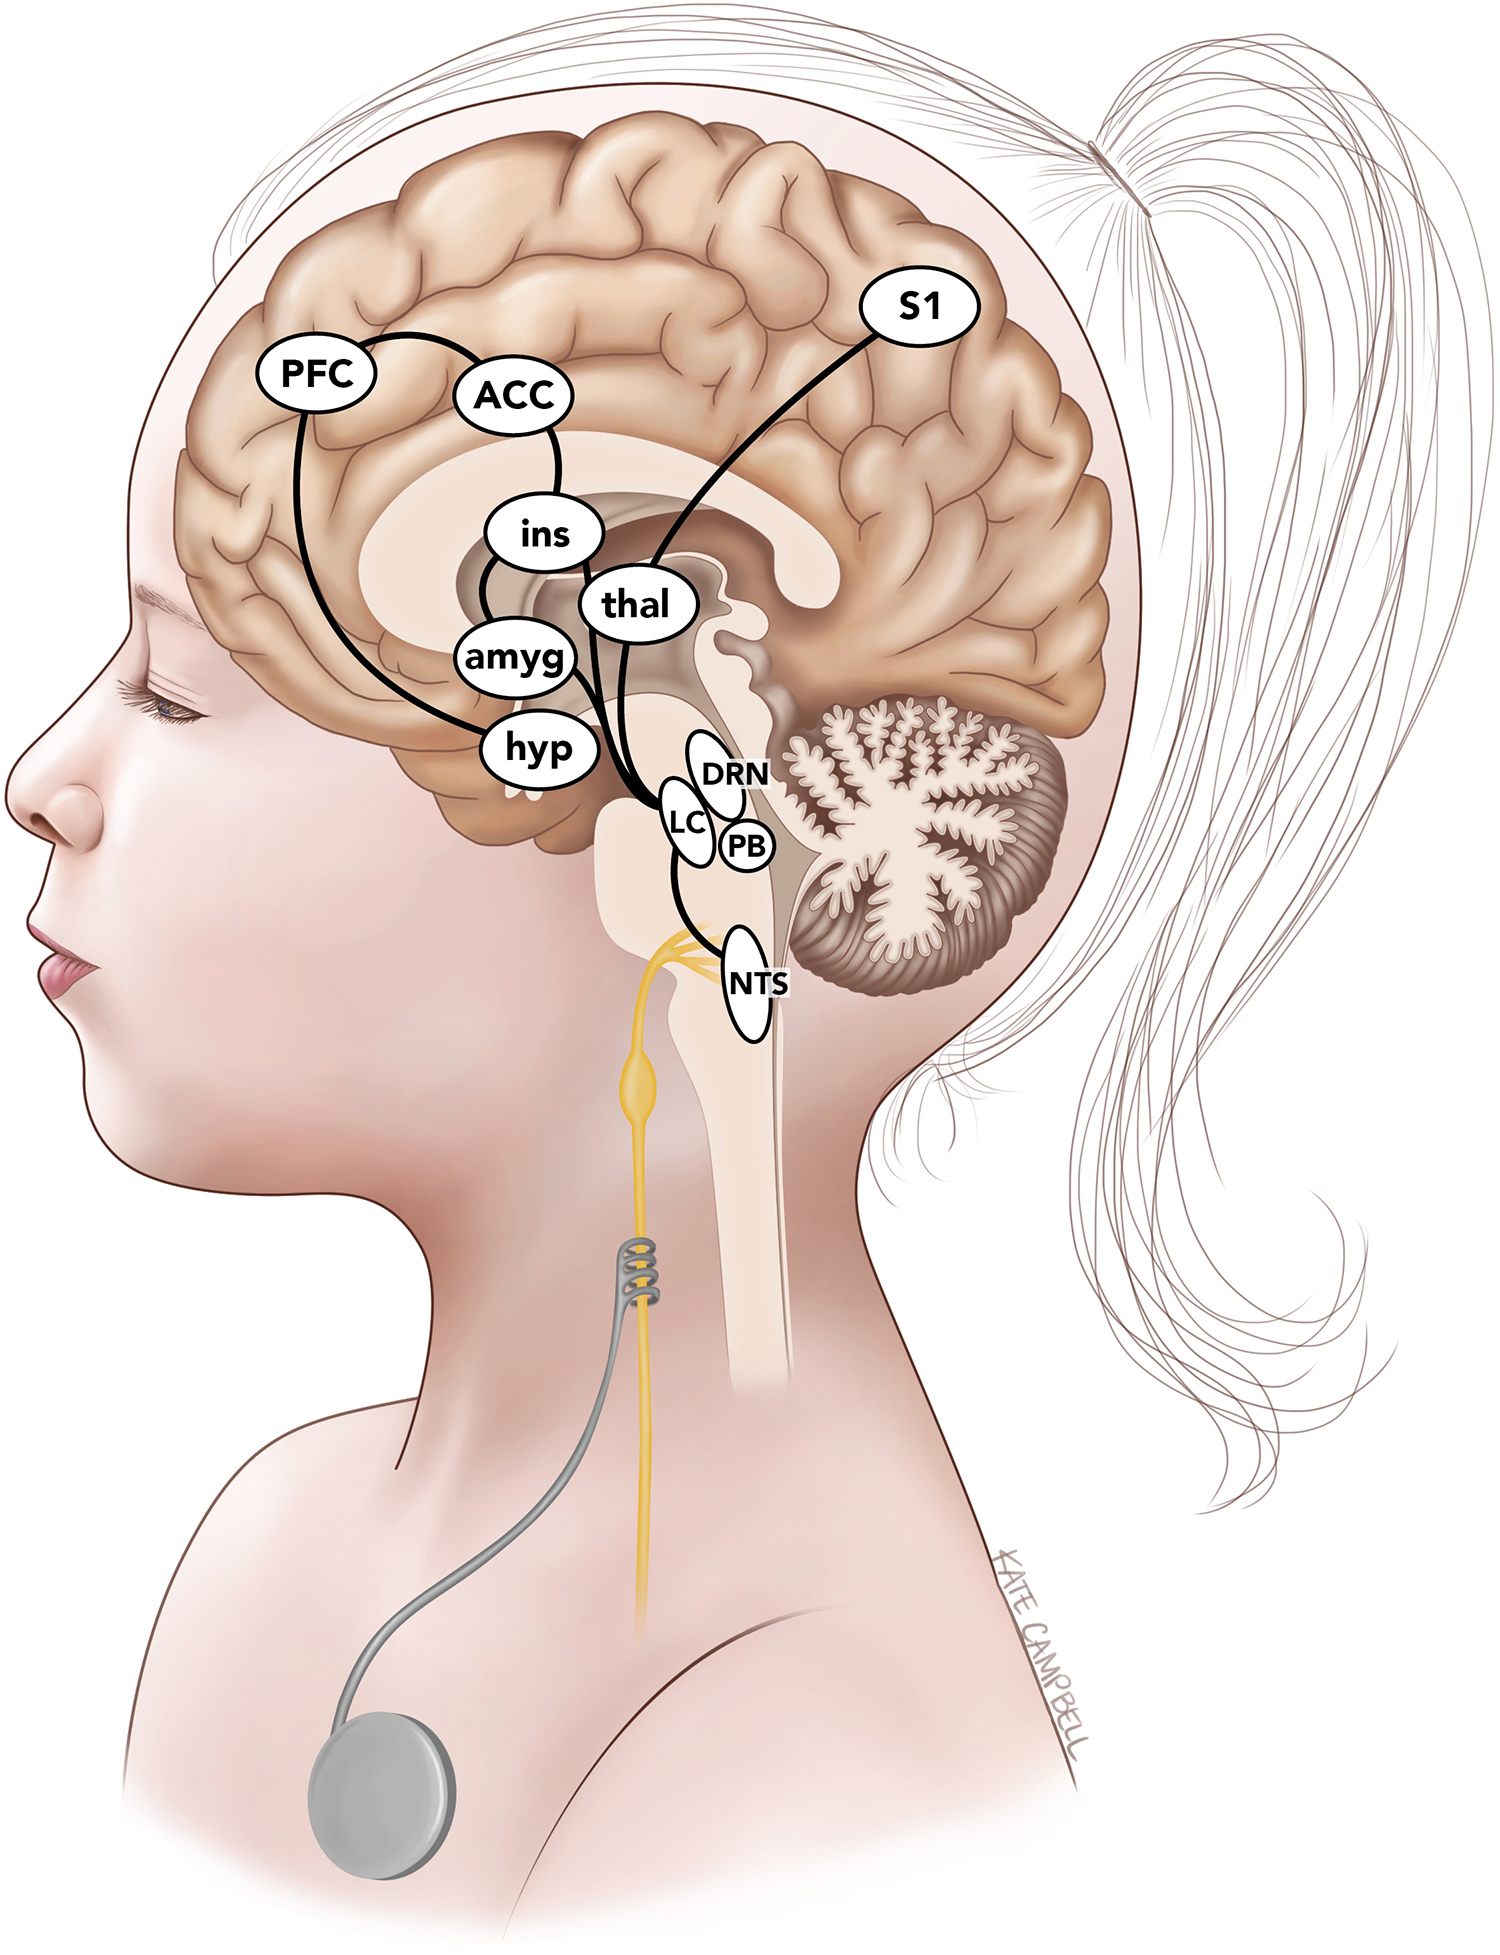
\includegraphics[width=\textwidth]{images/vagus_afferent_network.jpg}
    \end{minipage}\hfill
    \begin{minipage}[c]{0.5\textwidth}
      \caption{The vagus afferent network. Schematic diagram showing the important brainstem centers and subcortical and cortical structures. \cite{campbell, HanchemWongIbrahim2018}} 
      \label{fig:Vagus Afferent Network}
    \end{minipage}
    \centering
  \end{figure}

  The LC is characterized by widely diffused projections to both subcortical and cortical structures. The projections of the LC are small unmyelinated fibers, forming a wide antero-posterior branching network to reach the raphe nuclei, the cerebellum, and almost all areas of the midbrain and forebrain regions. The LC is the main source of norepinephrine (NE) in the brain \cite{AGHAJANIAN1977570}. NE is a neurotransmitter that has been associated with the clinical effects of VNS by preventing seizure development and by inducing long-term plastic changes that could restore a normal function of the brain circuitry. Indeed, short bursts of VNS increase neuronal firing in the LC, leading to elevations in NE concentrations. \cite{BergerVespa2021}

  Studies have demonstrated indirect projection of the LC to the DRN, which sends widespread projections to upper cortical regions. DRN appears to have a more delayed response to VNS \cite{HanchemWongIbrahim2018}.

  Vagal afferents project to the PBN by way of both the NTS and LC. Cell bodies within the PBN send diffuse outputs to forebrain structures including the thalamus, insular cortex, amygdala, and hypothalamus. Moreover, PBN likely plays an important role in regulating thalamocortical circuitry that may be implicated in seizure generation. Specifically, PBN activates the intralaminar nuclei of the thalamus, which in turn relays sensory signals to widespread cortical areas. \cite{HanchemWongIbrahim2018}

  \subsection*{The Vagus Afferent Network}
    \subsubsection*{Structural and Functional connectivity}
    Structural connectivity and functional connectivity are two concepts that describe different aspects of brain organization. Structural connectivity refers to the anatomical organization of the brain by means of fiber tracts that connect different brain regions \cite{sporns2022structure}. Functional connectivity refers to the statistical dependence or correlation of neural activity patterns between different brain regions \cite{GRAFTON2019237}. Structural connectivity is often measured by diffusion magnetic resonance imaging (dMRI). Functional connectivity is often measured by electro-encephalography (EEG) or functional magnetic resonance imaging (fMRI)\footnote{fMRI is a non invasive neuroimaging technique that detects the changes in blood oxygenation and flow that occur in response to neural activity} \cite{sporns2022structure}.

    The main difference between structural connectivity and functional connectivity is that structural connectivity reflects the physical architecture of the brain, while functional connectivity reflects the dynamic interactions of neural activity, as shown in Figure \ref{fig:Structural and Functional Connections}. Functional connectivity can emerge from direct or indirect structural connections, as well as from external inputs or intrinsic dynamics.

    \begin{figure}[h]
      \centering
      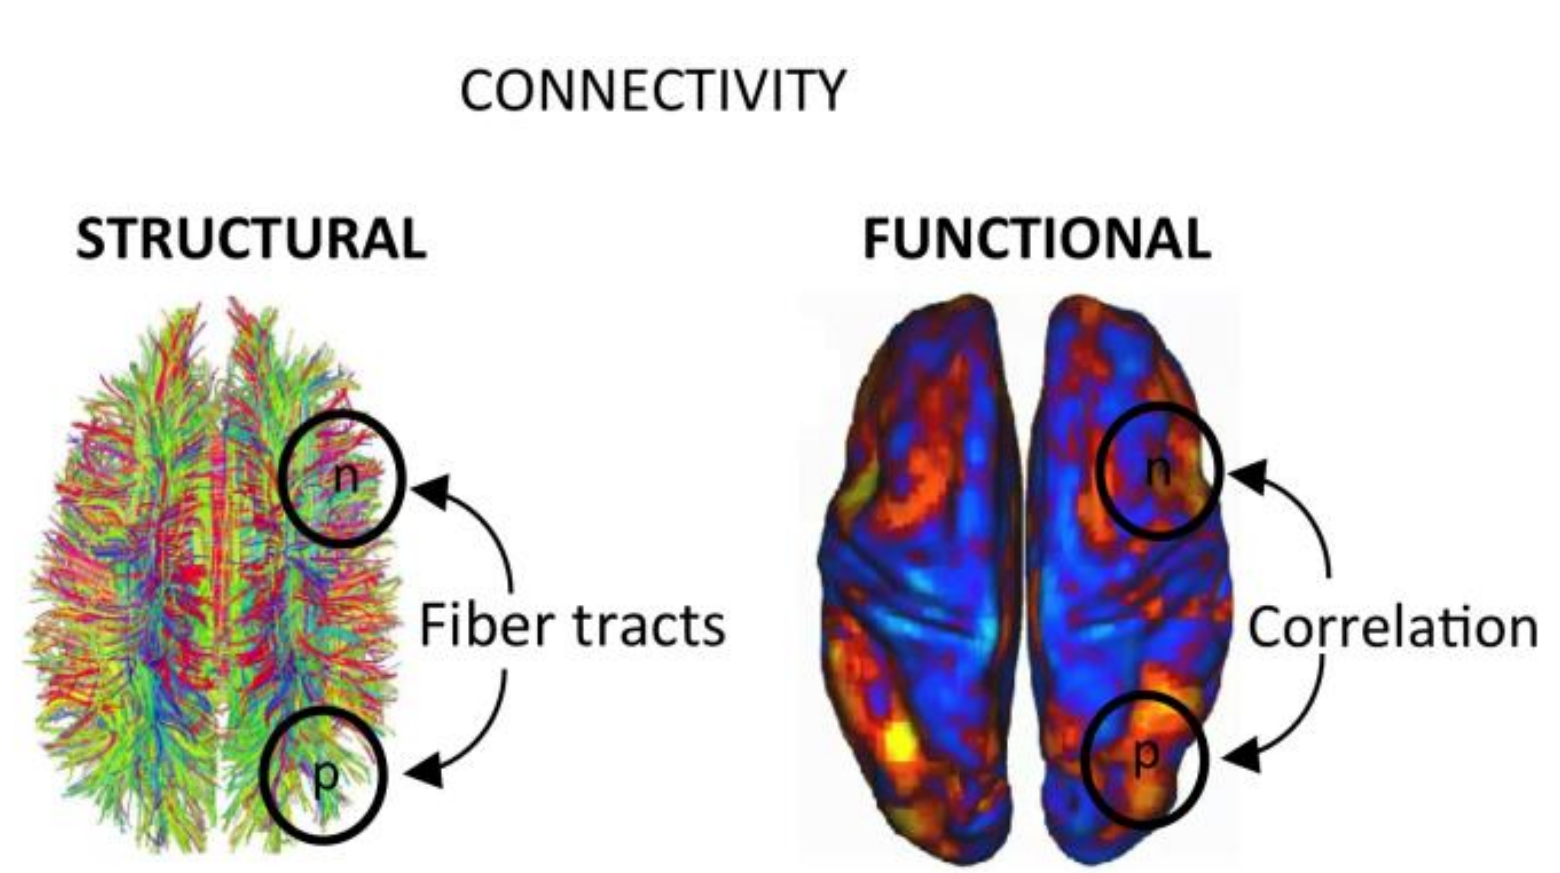
\includegraphics[width=0.8\textwidth]{images/structuralFunctional.png}
      \caption{Differences between structural and functional connectivity \cite{CABRAL201784}.}
      \label{fig:Structural and Functional Connections}
    \end{figure}

    \subsubsection*{Functional connectivity results in VNS}
    Recently, thalamic activation measured by BOLD fMRI was associated with improved VNS treatment response in patients with seizures \cite{NarayananWatts2002}. The importance of thalamocortical connections increased after a study that utilized resting-state functional MRI (rs-fMRI) data pre-VNS implantation and found an association of greater VNS efficacy with larger connectivity between the thalami to the anterior cingulate cortex (ACC) and left insular cortex \cite{IBRAHIM2017634}. 
    
    Functional connectivity in MEG\footnote{Magnetoencephalography: is a functional neuroimaging technique that maps brain activity by recording magnetic fields produced by electrical currents occurring naturally in the brain, using very sensitive magnetometers.} also supports the role of intrinsic thalamocortical connectivity in VNS responders, was found that a functional network is significantly more active in VNS responders \cite{Mithani2019, Mithani2020}. Specifically, fMRI studies in healthy individuals undergoing noninvasive VNS reported increased activity in the medial longitudinal fasciculus \cite{frangos2017access}.

    \subsubsection*{Structural connectivity results in VNS}
    Significantly greater FA was observed in VNS (lateralized to the left) responders particularly within anterior and retrolenticular limbs of the internal capsule, anterior, superior and posterior corona radiata, and posterior thalamic radiation \cite{Mithani2019}.

    In a study of 56 children done by \cite{Mithani2019} significantly greater FA (within the left size) was observed in VNS responders in the left internal capsule, external capsule, corona radiata, posterior thalamic radiation, fornix and stria terminalis, superior longitudinal fasciculus, inferior longitudinal fasciculus, and inferior front-occipital fasciculus. The mean FA value in these tracts was 0.352 (standard deviation SD = 0.048) in responders and 0.309 (SD = 0.064) in non responders. No significant voxels were observed in the right hemisphere. Furthermore, no statistically significant differences were observed in any other DTI parameters, including MD, radial diffusivity, and axial diffusivity. Healthy controls showed that the profile of responders was more closely related to healthy children than non responders. The mean FA value in significant tracts for matched controls was 0.377 (SD = 0.0274) in healthy controls. \cite{Mithani2019}.

    \noindent A study conducted on a 4-year-old boy with intractable epilepsy at 10 months after implantation of VNS showed increased FA in the right fimbria-fornix at the level of both cerebral peduncles. \cite{Fan2014}
  
  \subsection*{Tracts of interest}

    Thalamocortical connections are believed to be an important substrate of VNS responsiveness because they modulate cortical excitability, rendering the brain less susceptible to seizures. The thalamus receives direct inputs from the NTS and PBN \cite{BecksteadJoel2980}.

    The limbic system is a collection of neuronal structures involved in controlling emotion, memory, behavior, and motivation. The fornix is the main efferent tract of the hippocampus projecting to the mammillary bodies, nucleus accumbens, septal nuclei, anterior thalamic nuclei and cingulate cortex. While, the stria terminalis forms the major input tract from the amygdala to the hypothalamus.
    
    Association fibers link different cortical areas in the same hemisphere \cite{standring2005gray}. It is possible that they enable transmission of the modulatory stimulus to epileptogenic and/or symptomatogenic regions, which would be augmented by increased white matter microstructure in those tracts.

    \subsubsection*{Thalamocortical connections}
    

    \subsubsection*{Fornix and Stria Terminalis}
    The \emph{fornix} is apart of the limbic system and is a C-shaped bundle of nerve fibers that act as the major output tract of the hippocampus. \cite{Fornixof88:online}
    The \emph{stria terminalis} is a fasciculus of fibers running along the lateral margin of the thalamus. It is the major output pathway of the amygdala. \cite{DUDAS20211}
    Both fornix and stria terminalis are represented in Figure \ref{fig:fornixST}

    \begin{figure}[h]
      \centering
      \begin{minipage}[c]{0.6\textwidth}
        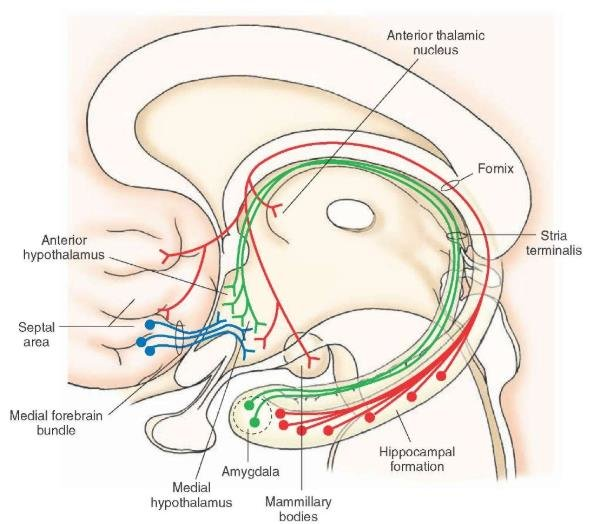
\includegraphics[width=\textwidth]{images/fornixST.jpg}
      \end{minipage}\hfill
      \begin{minipage}[b]{0.37\textwidth}
          \caption{Illustration of anatomical structure and boundaries of stria terminalis and fornix. \cite{alahmari2021}}
          \label{fig:fornixST}
      \end{minipage}
   \end{figure}
   
   \subsubsection*{Association Fibers}
   The \emph{superior longitudinal fasciculus} (SLF) is an association tract \ref{fig:SLF} in the brain that is composed of three separate components . The first (SLF I) is located in the white matter of the superior parietal and superior frontal lobes. The second, (SLF II) occupies the central core of the withe matter above the insula. While the last one, (SLF III) is situated in the white matter of the parietal and frontal opercula. \cite{10.1093/cercor/bhh186}

   The \emph{inferior longitudinal fasciculus} is an associative white matter pathway that connects the occipital and temporal-occipital areas to the anterior temporal areas as shown in Figure \ref{fig:ILF}. 

   \begin{figure}[h]
    \centering
    \begin{subfigure}{.5\textwidth}
      \centering
      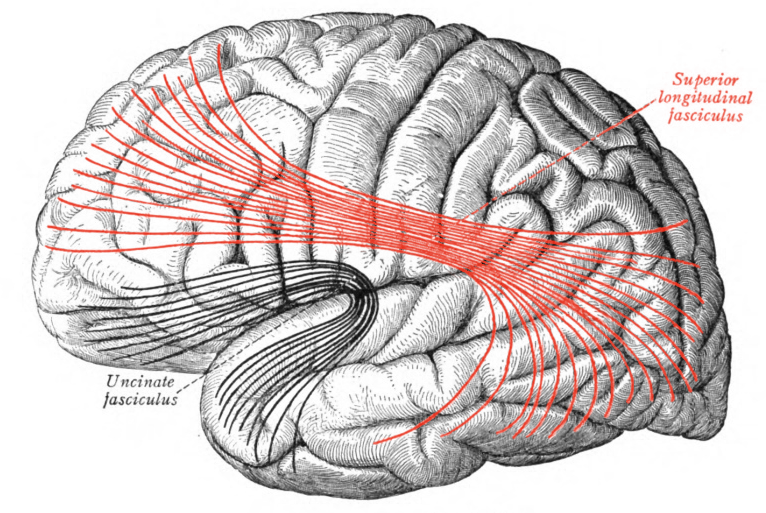
\includegraphics[width=0.95\linewidth]{images/SLF.png}
      \caption{}
      \label{fig:SLF}
    \end{subfigure}%
    \begin{subfigure}{.5\textwidth}
      \centering
      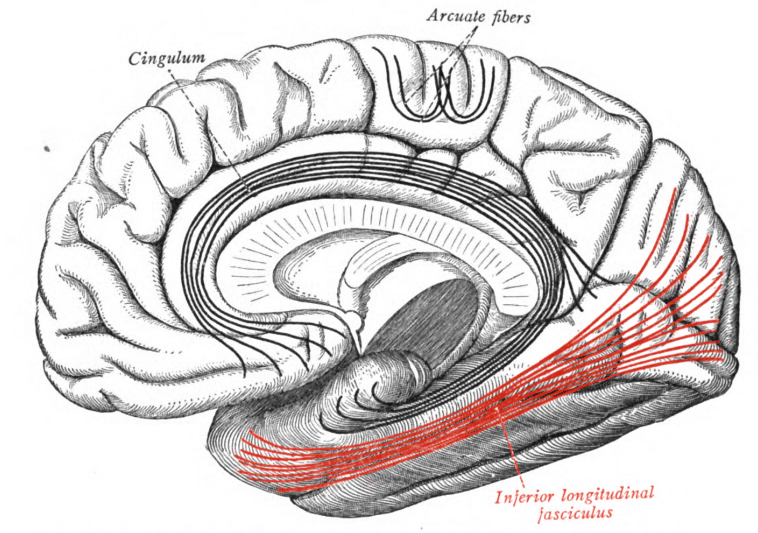
\includegraphics[width=0.95\linewidth]{images/ILf.png}
      \caption{}
      \label{fig:ILF}
    \end{subfigure}
    \caption{Representation of longitudinal fascicles: (a) Superior longitudinal fasciculus; (b) Inferior longitudinal fasciculus. \cite{sobottaAtlas1908}}
 \end{figure}
  



  
  \chapter{Methods}
  \section{Data}
 \subsection{Subjects}
 % Sempre sulla falsa riga di Raskin, mi piace il su stile

 % Number of subjects

 % Demographic table

 % Others...
 \subsection{Data acquisition}
 The MRI acquisitions were realized following the \emph{LivaNova guidelines}, requiring the neurostimulators to be turned off during the acquisitions. A trained neurologist used the programming system to set the output current of the device to 0 mA and turn off the sensing before that the patients entered the MRI acquisition room. 

 Imaging data were acquired using the \emph{SIGNA\textsuperscript{\texttrademark} Premier 3T MRI} system (GE Healthcare, Milwaukee, WI, USA), with a transmit-receive 48-channel head coil. \\ T1-anatomical images were acquired using a \emph{Magnetization Prepared - RApid Gradient Echo} (MPRAGE) sequence with the following parameters: $TR = 2186 ms$, $TE = 2.95 ms$, $FA = 8^{\circ}$, $TI = 900 ms$, bandwidth = $244.14 Hz$, matrix size = 256 x 256, 156 axial slices, imaging frequency = $127.77 Hz$, voxel size = 1 x 1 x 1 $mm^3$, acquisition time = 5:26 min.

 Diffusion MRI data were acquired with a \emph{Pulsed Gradient Spin Echo} (PGSE) sequence with the following parameters : $TR = 4837 ms$, $TE = 80.5 ms$ and flip angle = $90^{\circ}$. A multi-shell diffusion scheme was used and was composed of 64 gradients at b = 1000, and 32 gradients at b = 2000, 3000 and 5000 $[s \cdot mm^{-2}]$, interleaved with 7 b0 images. The in-plane FOV was 220 x 220 $mm^{2}$ and the data contained 68 axial slices with a $2 mm$ thickness (no inter-slice gap, $2 mm$ isotropic voxels). A multi-slice excitation scheme was used during the acquisition with a hyperband slice factor of 3 to reduce the acquisition time. The total acquisition time was 13:33 min.

 Anatomical files are composed of a NIfTI file (\texttt{.nii.gz}) \ref{fig:T1_images} containing the measured signal and a JSON file (\texttt{.json}) regrouping the acquisition sequence parameters.
 % TODO put the figure of the brain view of T1 and T2 images from sagittal frontal and axial view

 \begin{figure}[h]
    \centering
    %\includegraphics[width=0.8\textwidth]{}
    \caption{Anatomical volume slices of a T1 in the sagittal, frontal and axial views}
    \label{fig:T1_images}
  \end{figure}

  \begin{figure}[h]
    \centering
    %\includegraphics[width=0.8\textwidth]{}
    \caption{Anatomical volume slices of a T2 in the sagittal, frontal and axial views}
    \label{fig:T1_images}
  \end{figure}

 Diffusion files are composed of a NIfTI file and a JSON file plus two text files (\texttt{.bval}) and (\texttt{.bvec}) containing the b-values and the b-vectors.
 % TODO put the figure of the diffusion image at different b-values

 \begin{figure}[h]
    \centering
    %\includegraphics[width=0.8\textwidth]{}
    \caption{Raw diffusion volume slices of a patient for different b-values}
    \label{fig:DwMri_images}
  \end{figure}
 
\section{Data preprocessing}
\section{Tractography}
%\subsection{Evaluation of Tractography}
\section{Microstructural analysis}
\section{Statistical analysis}

  \chapter{Results}

  \chapter{Discussion}

  \addcontentsline{toc}{chapter}{Conclusion and perspectives}
  \chapter*{Conclusion and perspectives}
  
  \bibliographystyle{apalike}
  \bibliography{refs}

  % Back cover page
  \backcoverpage

\end{document}
